\documentclass[10 pt,usenames,dvipsnames, oneside]{article}
\usepackage{../../../modelo-ensino-medio}


\begin{document}

\begin{center}
  \begin{minipage}[l]{3cm}
\includegraphics[width=2cm]{logo}    
\end{minipage}\hfill
\begin{minipage}[r]{.8\textwidth}
 {\Large \scshape Atividade: Uma Viagem de Carro}  
\end{minipage}
\end{center}
\vspace{.2cm}

\ifdefined\prof
\begin{objetivos}
\item \textbf{LAF3} Calcular e interpretar a taxa de variação média de uma função em um intervalo dado, tanto algebricamente quanto a partir de dados gráficos ou de uma tabela, identificando tendências de crescimento e decrescimento.
\end{objetivos}

\begin{goals}
\begin{enumerate}

\item [OE1] Interpretar, em uma situação concreta, o conceito de velocidade média e suas particularidades.

\item [OE2] Representar graficamente (tabela e sistema de coordenadas) as informações do problema.

\end{enumerate}

\tcblower
\begin{itemize}
\item A escolha dessa atividade se deu pelo fato de podermos usar o conceito de velocidade
média (que é mais intuitivo e que o estudante já teve contato na disciplina de Física)
como base para a generalização de taxa de variação média de uma função qualquer.
\end{itemize}
\end{goals}

\bigskip
\begin{center}
{\large \scshape Atividade}
\end{center}
\fi

Você está viajando de carro para uma cidade que está a 410 km de distância da sua casa. Você sai ao meio dia e depois de 2h de viagem faz a primeira parada em um posto de combustível na estrada. Olhando no GPS, calcula que já percorreu 140 km desde a sua partida. Depois de 30 minutos parte para a estrada novamente. Faz uma nova parada das 16h às 16h30 em outro posto 120 km adiante do anterior. E finalmente às 18h chega ao seu destino.

\begin{enumerate}
\item Preencha a tabela abaixo com as distâncias percorridas e marque no sistema de coordenadas os pares ordenados correspondentes (o eixo horizontal representa o tempo decorrido em horas desde a partida e o eixo vertical a distância percorrida em quilômetros).

\begin{table}[H]
\centering
\begin{tabu} to \textwidth{|r|c|c|}
\hline
\thead
Horário & \parbox{3.5cm}{\centering\vspace{.5em} Tempo decorrido desde a partida (h)\vspace{.5em}} & \parbox{3.5cm}{\centering\vspace{.5em} Distância percorrida (km)\vspace{.5em}} \\
\hline
& t & d(t) \\
\hline
12h & 0 & \\
\hline
14h & 2 & \\
\hline
14h30 & 2.5 & \\
\hline
16h & & \\
\hline
16h30 & & \\
\hline
18h & & \\
\hline
\end{tabu}
\end{table}

\begin{figure}[H]
\centering
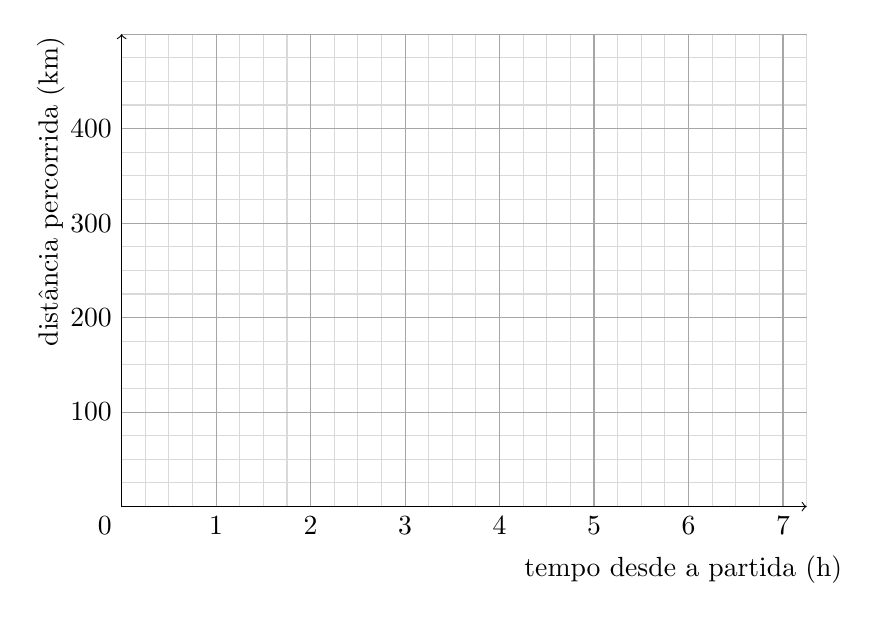
\begin{tikzpicture}[scale=1.2]

\draw [gray!30, step=.25] (0,0) grid (7.25,5);
\draw [gray!70] (0,0) grid (7.25,5);
\draw [->] (0,0) -- (7.25,0) node [below, shift={(0,-.5)}, pos=.82] {tempo desde a partida (h)};
\draw [->] (0,0) -- (0,5) node [pos=.75,above, rotate=90, shift={(-.5,.6)}] {distância percorrida (km)};
\foreach \x in {1,...,7} \node [below] at (\x,0) {\x};
\foreach \x in {1,...,4} \node [left] at (0,\x) {\x00};
\node [below left] at (0,0) {0};

\end{tikzpicture}
\end{figure}
\item A distância total percorrida na viagem foi de 410 km, e durou 6h. Podemos obter a \textbf{velocidade média} da viagem dividindo esses dois valores, obtendo
\begin{equation*}
\frac{\Delta d}{\Delta t}=\frac{410}{6}=51,5 \cdot \frac{km}{h}
\end{equation*}
O que representa esse número no contexto do problema?
\item Calcule a velocidade média para o trecho da partida até chegar à primeira parada
\begin{equation*}
\frac{\Delta d}{\Delta t}=\cdot=\frac{km}{h}
\end{equation*}
Ele é o mesmo que o anterior? Explique
\item Sem fazer a conta, você imagina que o valor da velocidade média no trecho da partida até a hora de sída a primeira parada (14h30) será maior ou menor que o valor do item anterior? Por que?
\item Preencha a tabela com as velocidade médias nos trechos indicados.

\begin{table}[H]
\centering
\setlength\tabulinesep{1mm}
\begin{tabu} to \textwidth{|c|c|}
\hline
\thead
Intervalo de tempo $a,b$ & \makecell{Velocidade média \vspace{.3em}\\  $\bm{\displaystyle \frac{\Delta d}{\Delta t} = \frac{d(b)-(d(a)}{b-a}}$} \\
\hline
$0,2$ & \\
\hline
$2,2.5$ & \\
\hline
$2.5,4$ & \\
\hline
$4,4.5$ & \\
\hline
$4.5,6$ & \\
\hline
\end{tabu}
\end{table}
\end{enumerate}

\ifdefined\prof

\clearpage
\begin{solucao}
\begin{enumerate}
\item \adjustbox{valign=t}{
\centering
\begin{tabu} to \textwidth{|c|c|c|}
\hline
\thead
Horário & \makecell{Tempo decorrido \\ desde a partida (h)} & \makecell{Distância percorrida \\ (km)} \\
\hline
& $t$ & $d(t)$ \\
\hline
12h & 0 & 0 \\
\hline
14h & 2 & 140 \\
\hline
14h30 & 2.5 & 140 \\
\hline
16h & 4 & 260 \\
\hline
16h30 & 4.5 & 260 \\
\hline
18h & 6 & 410 \\
\hline
\end{tabu}
}
\vspace{2em}
\begin{figure}[H]
\centering
\begin{tikzpicture}[scale=1.2, every node/.style={black},every path/.style={black}]

\draw [gray!30, step=.25] (0,0) grid (7.25,5);
\draw [gray!70] (0,0) grid (7.25,5);
\draw [->] (0,0) -- (7.25,0) node [below, shift={(0,-.5)}, pos=.82] {tempo desde a partida (h)};
\draw [->] (0,0) -- (0,5) node [pos=.75,above, rotate=90, shift={(-.5,.6)}] {distância percorrida (km)};
\foreach \x in {1,...,7} \node [below] at (\x,0) {\x};
\foreach \x in {1,...,4} \node [left] at (0,\x) {\x00};
\node [below left] at (0,0) {0};

\coordinate (a) at (0,0);
\coordinate (b) at (2,1.4);
\coordinate (c) at (2.5,1.4);
\coordinate (d) at (4,2.6);
\coordinate (e) at (4.5,2.6);
\coordinate (f) at (6,4.1);

\foreach \x in {a,b,c,d,e,f} \fill [session3] (\x) circle (2pt);

\draw [dashed, session3] (a) -- (b) -- (c) -- (d) -- (e) -- (f);
\end{tikzpicture}
\end{figure}

\item Que, em média, a cada hora a distância percorrida foi de $51,5$ km. Ou que se tivesse sido mantida uma velocidade constante ao longo de toda viagem (sem paradas) esse deveria ser o valor para se chegar ao mesmo tempo no destino.

\item $\displaystyle\frac{\Delta d}{\Delta t}= \frac{140}{2}=70\frac{km}{h}$. O valor da velocidade média neste trecho é maior que o anterior. Em média, o carro andou mais rápido durante a primeira parte da viagem do que na viagem toda, fazendo $70$ km a cada hora.

\item Será menor, pois o carro passou 30 minutos parado, o que diminui a velocidade média. Em termos da conta, mantém-se o numerador e aumenta-se o denominador, gerando um número menor.

\clearpage
\item \adjustbox{valign=t}{
\begin{minipage}{\linewidth}
\setlength\tabulinesep{2.5pt}
\begin{tabu} to \textwidth{|c|c|}
\hline
\thead
Intervalo de tempo $\bm{[a,b]}$ & Velocidade média $\displaystyle\bm{\frac{\Delta d}{\Delta t}=\frac{d(b)-d(a)}{b-a}}$\\
\hline
$[0,2]$ & $\displaystyle\frac{\Delta d}{\Delta t}=\frac{140}{2}=70 km/h$ \\
\hline
$[2,2.5]$ & $\displaystyle\frac{\Delta d}{\Delta t}=\frac{0}{0,5}=0 km/h$ \\
\hline
$[2.5,4]$ & $\displaystyle\frac{\Delta d}{\Delta t}=\frac{120}{1,5}=80 km/h$ \\
\hline
$[4,4.5]$ & $\displaystyle\frac{\Delta d}{\Delta t}=\frac{0}{0.5}=0 km/h$ \\
\hline
$[4.5,6]$ & $\displaystyle\frac{\Delta d}{\Delta t}=\frac{150}{1,5}=100 km/h$ \\
\hline
\end{tabu}
\end{minipage}
}

\end{enumerate}

\end{solucao}
\fi

\end{document}